\providecommand{\main}{..}
\documentclass[\main/notes.tex]{subfiles}

\begin{document}
	\setcounter{chapter}{12}
	\chapter{File Structure}
		Files are stored on \concept{auxilary} or \concept{secondary storage devices}. The two most common forms are disk and tape. Files in secondary storage can be both read from and written to. Other files can be written to, but not read from.
		\begin{definition}{File}
			A collection of data records in which each record consists of one or more fields.
		\end{definition}
		\begin{definition}{Access Method}
			How records are accessed or retrieved from a file: \concept{sequentially} or \concept{randomly}.
			\begin{center}
				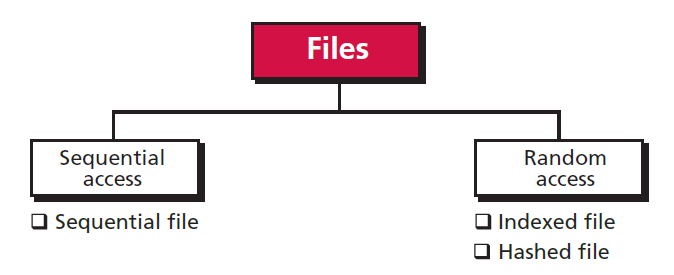
\includegraphics[width=0.6\textwidth]{\main/images/unit13/taxonomy.png}
			\end{center}
			\begin{description}
				\item[Sequential Access] Access one record after another, from beginnng to end. Use a \concept{sequential file structure}.
				\item[Random Access] Access a specific record without having to retrieve all recourds before it. Can be done with structures such as \concept{indexed files} and \concept{hashed files}.
			\end{description}
		\end{definition}
		\pagebreak
		\section{Sequential Files}
			\begin{definition}{Sequential File}
				A file where records can only be accessed one after another from beginning to end. There is an \concept{EOF (end-of-file) marker} after the last record. The operating system has no information about the record addresses, it only knows where the whole file is stored.
				\begin{center}
					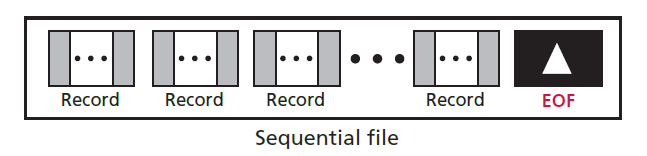
\includegraphics[width=0.6\textwidth]{\main/images/unit13/sequential_file.png}
				\end{center}
			\end{definition}
			Used in applications where all records need to be accessed from beginning to end. Not efficient for random access.
			\subsection{Updating Sequential Files}
				Four files associated with an update program: the \concept{new master file}, the \concept{old master file}, the \concept{transaction file}, and the \concept{error report file}. All these files are stored based on key values.
				\begin{indentparagraph}
					\begin{description}
						\item[New Master File] Contains the most current data. Also called the \concept{new permanent data file}.
						\item[Old Master File] The previous version of the master file, that should be updated. Normally kept for reference.
						\item[Transaction File] Contains the changes to be applied to the master file. There are three basic types.
							\begin{indentparagraph}
								\begin{description}[nosep]
									\item[Add transactions] Contain data about a new record to be added to the master file.
									\item[Delete transations] Identify records to be deleted from the file.
									\item[Change transcations] Contain revisions to specific records in the file.
								\end{description}
							\end{indentparagraph}
							To perform a transaction, a \concept{key} is needed. A \concept{key} is one or more fields that uniquely identify the data in the file.
						\item[Error Report File] A listing of all errors discovered during the update process.
					\end{description}
				\end{indentparagraph}
				\subsubsection{Processing File Updates}
					\begin{enumerate}[nosep]
						\item If the transaction file key is less than the master file key, and the transaction is an add (A), add the transaction to the new master.
						\item If the transaction file key is equal to the master file key, either:
						\begin{enumerate}[nosep]
							\item Change the contents of the master file if the transaction is a change (C).
							\item Remove the data from the master file if the transaction is a delete (D).
						\end{enumerate}
						\item If the transaction file key is greater than the master file key, write the old master file record to the new master file.
					\end{enumerate}
					Some cases that might cause an error are:
					\begin{enumerate}[nosep]
						\item If the transaction defines adding a record that already exists in the old master file (same key values).
						\item If the transaction defines deleting or changing a record that does not exist in the old master file.
					\end{enumerate}

		\section{Indexed Files}
			Used to access a record in a file randomly. The address of the record needs to be known.
			\begin{definition}{Indexed File}
				Made of a \concept{data file} (a sequential file), and an \concept{index}. The index is a small file with two fields: the key of the data file, and the address of the corresponding record on disk.

				\begin{center}
					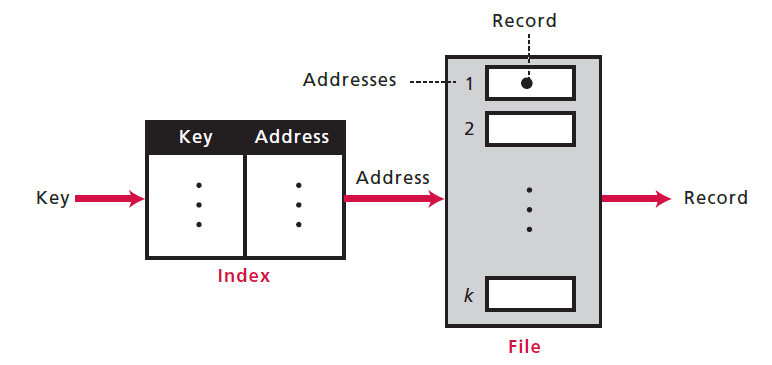
\includegraphics[width=0.6\textwidth]{\main/images/unit13/indexed_file_mapping.png}
				\end{center}

				An example:
				\begin{center}
					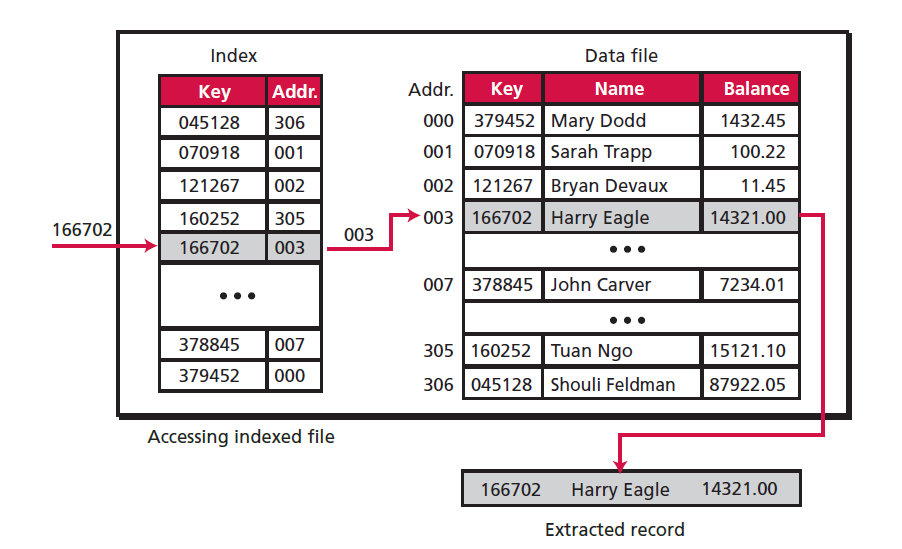
\includegraphics[width=0.7\textwidth]{\main/images/unit13/indexed_file_example.png}
				\end{center}
			\end{definition}
			\begin{enumerate}[nosep]
				\item Load the entire index file into memory
				\item The index entries are searched using an efficient search algorithm
				\item The address of the record is retrieved
				\item Using the address, the data record is retrieved, and passed to the user.
			\end{enumerate}
			\subsection{Inverted Files}
				\begin{definition}{Inverted File}
					Have more than one index for a file, with different keys.
				\end{definition}

		\section{Hashed Files}
				\begin{definition}{Hashed File}
					Uses a mathematical function to accomplish the mapping of a key to an address. A user gives the key, the function maps the key to the address and passes it to the operating system, and the record is retrieved.
					\begin{center}
						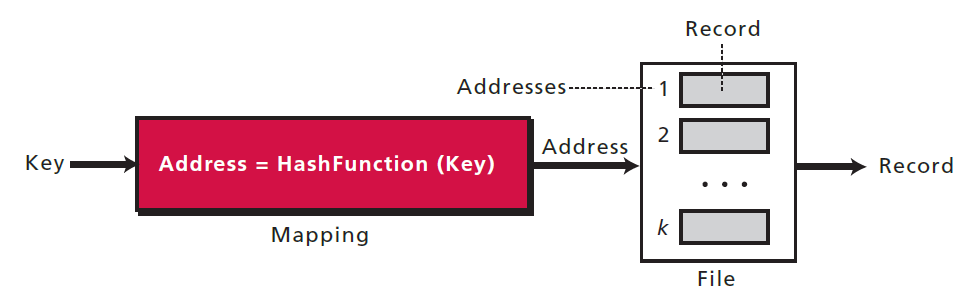
\includegraphics[width=0.8\textwidth]{\main/images/unit13/hashed_file_mapping.png}
					\end{center}
				\end{definition}
			\subsection{Hashing Methods}
				\begin{definition}{Direct Hashing}
					The key is the data file address without any algorithmic manipulation. The file must therefore contain a record for every possible key.

					Guarantees no \concept{synonyms} or \concept{collisions}.

					Limited applications, as inefficent to store this many records.

					\begin{center}
						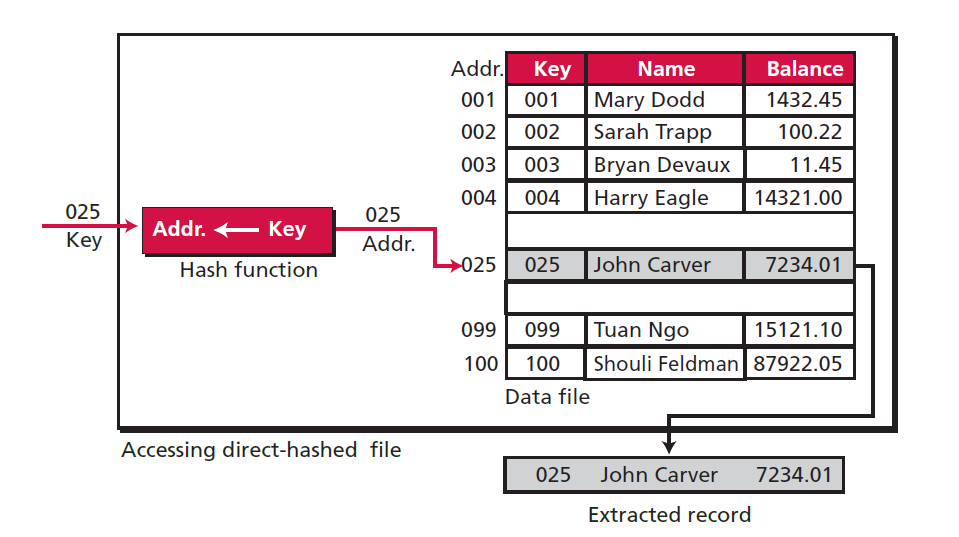
\includegraphics[width=0.8\textwidth]{\main/images/unit13/direct_hash_example.png}
					\end{center}
				\end{definition}
				\pagebreak
				\begin{definition}{Modulo division hashing}
					Also known as \concept{division remainder hashing}. Divides the key by the file size and uses the remainder plus $1$ for the address. \texttt{listSize} is the number of elements in the file.
					\begin{align*}
						\mathtt{address} &= (\mathtt{key} \text{ mod } \mathtt{listSize}) + 1
					\end{align*}
					Adding $1$ to the modulo operation, as the list starts with $1$ instead of $0$.

					Works with any list size, but a list size that is a \emph{prime number} produces less collisions.

					\begin{center}
						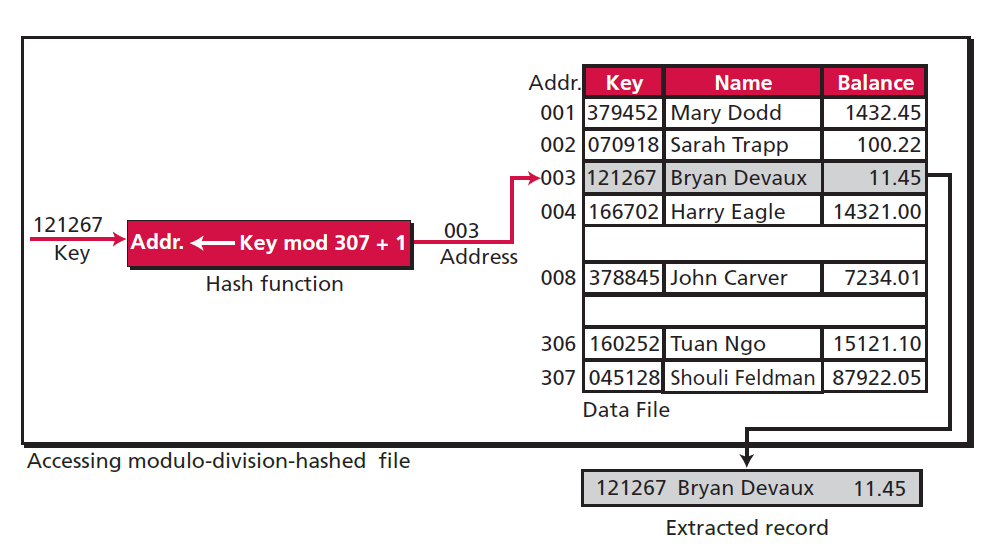
\includegraphics[width=0.8\textwidth]{\main/images/unit13/modulo_hash_example.png}
					\end{center}
				\end{definition}
				\begin{definition}{Digit Extraction Hashing}
					Selected digits are extracted from the key, and used as the address.

					As an example, map a $6$ digit number to a three-digit address, using the first, third and fourth digits.
					\begin{center}
						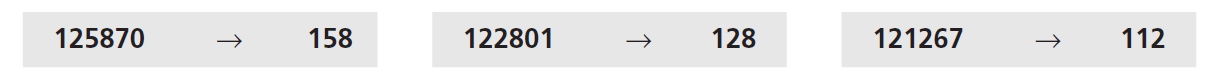
\includegraphics[width=0.8\textwidth]{\main/images/unit13/digit_hash_example.png}
					\end{center}
				\end{definition}
				Other methods exist, such as \concept{midsquare}, \concept{folding}, \concept{rotational}, and \concept{pseudorandom}.
			\pagebreak
			\subsection{Collision}
				\begin{definition}{Synonym}
					A key that hashes to the same address as another key.
				\end{definition}
				\begin{center}
					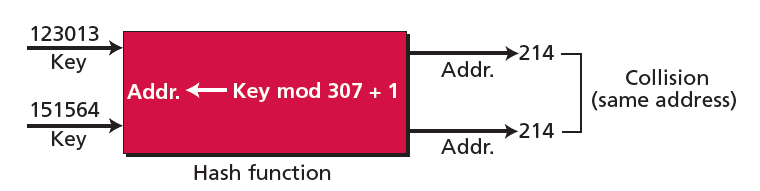
\includegraphics[width=0.6\textwidth]{\main/images/unit13/collision_example.png}
				\end{center}
				\begin{definition}{Collision}
					The event that occurs when a hashing algorithm produces an address for an insertion key, but that address is already occupied.
					\begin{indentparagraph}
						\begin{description}
							\item[Home address] Address produced by the hashing algorithm
							\item[Prime Area] Part of the file that contains all the home addresses 
						\end{description}
					\end{indentparagraph}
					When collision occurs at the home address, the collision is resolved by placing one of the keys and its data in a location outside the prime area.
				\end{definition}
				\subsubsection{Collision Resolution}
					Other than direct hashing, none of the methods assure that there is no collision. To resolve the potential collisions, different methods can be used.
					\begin{definition}{Open Addressing}
						Resolves collisions in the prime area. When a collision occurs, the prime area addresses are searched for an open or unoccupied record where the new data can be placed.

						However, this increases the probability of future collisions.
					\end{definition}
					\begin{definition}{Linked List Resolution}
						The first record is stored in the home address, but contains a pointer to the second record.
					\end{definition}
					\begin{definition}{Bucket Hashing}
						Create \concept{buckets} -- nodes that can accomodate more than one record. The disadvantage is that there may be a lot of unoccupied (wasted) locations within the prime area.
					\end{definition}
					A complex, effective mechanism for collision resolution will often use multiple approaches.

		\section{Directories}
			\begin{definition}{Directory}
				A mechanism for organising files. In most OSes, represented as a special type of file that holds information about other files. Serves as a kind of index that tells the OS where files are located on an auxilary storage device. Contains other information about the files, such as who has acces, or the date when each file was created, accessed, or modified.

				Generally organised in a tree structure, where each directory except the root has a parent. A directory in another directory is called a \concept{subdirectory}.
			\end{definition}
			\subsection{Directories in UNIX}
				\begin{description}
					\item[Root directory] Highest level of the file hierarchy. Does not have a parent directory. Belongs to the system admin, and can be changed only by the system admin.
					\item[Home directory] Accessed when a user first logs into a system. Contains files that are created when in the directory, which may include personal system files. Each user has a home directory.
					\item[Working Directory] Also called \concept{current directory}, or \concept{current working directory}. The directory a user is located at, at any point in a user session.
					\item[Parent Directory] The directory immediately above the working directory.
				\end{description}
			\subsection{Paths and Pathnames}
				To uniquely identify a file, specify the path from the root directory. This is known as the \concept{absolute pathname}. You can also specify a path relative to the current directory, which is known as a \concept{relative pathname}.

		\section{Text versus Binary}
			\subsection{Text Files}
				\begin{definition}{Text File}
					A file of characters. Does not contain any data structures, such as integers or floating-poing numbers.
				\end{definition}
			\subsection{Binary Files}
				\begin{definition}{Binary File}
					A collection of data stored in the internal format of the computer. Data can bne an integer, a floating-point number, or any other structured data (except a file).

					Data is only meaningful if properly interpreted by a program.
				\end{definition}

	\rulechapterend
\end{document}